%% LyX 2.3.6.1 created this file.  For more info, see http://www.lyx.org/.
%% Do not edit unless you really know what you are doing.
\documentclass[english]{article}
\usepackage[T1]{fontenc}
\usepackage[latin9]{inputenc}
\usepackage{geometry}
\geometry{verbose,tmargin=2.5cm,bmargin=2.5cm,lmargin=2.5cm,rmargin=2.5cm}
\usepackage{graphicx}

\makeatletter

%%%%%%%%%%%%%%%%%%%%%%%%%%%%%% LyX specific LaTeX commands.
%% Because html converters don't know tabularnewline
\providecommand{\tabularnewline}{\\}

\makeatother

\usepackage{babel}
\begin{document}
{[}SPLIT\_HERE{]}
\begin{enumerate}
\item \textbf{{[}DHS/PRELIM/9597/2014/P2/Q1{]} }

The Pioneer Generation Joint Committee (PGJC) is a diverse taskforce
set up to manage and promote information about the Pioneer Generation
Package (PGP) to honour and thank pioneers for their hard work and
dedication to make Singapore what it is today. The PGP will benefit
about 450,000 Singaporeans. 

Beyond the conventional means of raising awareness of PGP via mainstream
media (newspapers and television broadcast), PGJC also desires to
enhance its outreach using the Internet, new media (e.g. social networks)
and mobile applications. 
\begin{enumerate}
\item Give two advantages of using the latter modes of outreach compared
to traditional mass media. \hfill{}{[}2{]}
\item A significant challenge of using non-conventional outreach methods
is that while the Internet and mobile devices are becoming increasingly
ubiquitous, many user interfaces are often not well suited to the
elderly's specific needs. 

Design and justify an appropriate user interface for a pioneer to
enter information to file for hospitalisation claim on an insurance
company's website using a desktop or laptop computer. The information
required are: NRIC, hospital name, from and to dates of hospitalisation,
invoice number, invoice amount and brief description of reason for
hospitalisation. \hfill{}{[}4{]}
\item Give two factors developers would need to consider to adapt the user
interface for a mobile device such as a smartphone. \hfill{}{[}2{]}
\item The development of the PGP mobile application will involve the following
phases: 
\noindent \begin{center}
\begin{tabular}{|c|l|c|c|}
\hline 
Phase & Description & Duration(mandays) & Preceding Phase\tabularnewline
\hline 
\hline 
A & Adapt contents for smaller form factors & 8 & -\tabularnewline
\hline 
B & Prepare development environment & 2 & A\tabularnewline
\hline 
C & Purchase developer license (include approval time)  & 2 & B\tabularnewline
\hline 
D & Develop and test for Android & 4 & C\tabularnewline
\hline 
E & Develop and test for iOS & 3 & C\tabularnewline
\hline 
F & Publish to Google Play & 1 & D\tabularnewline
\hline 
G & Publish to App Store & 5 & E\tabularnewline
\hline 
H & Promotion and marketing & 3 & F, G\tabularnewline
\hline 
\end{tabular}
\par\end{center}
\begin{enumerate}
\item Construct a PERT chart for this project.\hfill{} {[}3{]}
\item State the critical path and the total time required for the project.\hfill{}
{[}2{]}
\item There is also a need to maintain documentation for the project. Why
is documentation important? \hfill{}{[}2{]}
\item Construct a Gantt chart to include and justify a documentation phase
of a reasonable duration.\hfill{} {[}3{]}
\end{enumerate}
\end{enumerate}
The following screenshot shows the user interface where a pioneer
can verify his/her eligibility. 
\noindent \begin{center}
<INSERT\_IMAGE\_HERE>
\par\end{center}
\begin{enumerate}
\item[(e)]  The code below the NRIC field shows a randomly generated string. 
\begin{enumerate}
\item Explain the purpose of this code. \hfill{}{[}1{]}
\item Outline an algorithm to generate another random string when the refresh
button is clicked.\hfill{} {[}3{]}
\end{enumerate}
\item[(f)]  Using examples from the above user interface, explain the following
concepts: 
\begin{enumerate}
\item (i) validation and verification \hfill{}{[}4{]}
\item (ii) client-side and server-side scripting \hfill{}{[}4{]}
\end{enumerate}
\item[(g)]  Information is transmitted to the server using the https protocol.
\begin{enumerate}
\item Explain the significance of this protocol.\hfill{} {[}2{]}
\item Describe how information is typically transmitted between a client
and a server. \hfill{}{[}3{]}
\end{enumerate}
\end{enumerate}
{[}SPLIT\_HERE{]}
\item \textbf{{[}DHS/PRELIM/9597/2014/P2/Q2{]} }

The following invoice shows the medical bill incurred by a pioneer
in a polyclinic. 
\begin{center}
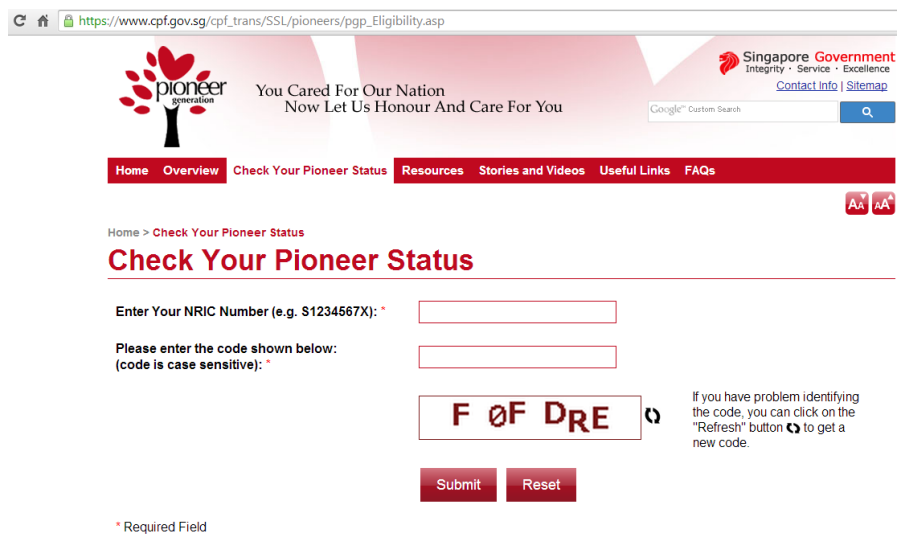
\includegraphics[width=0.65\paperwidth]{C:/Users/Admin/Desktop/Github/question_bank/LyX/static/img/9597-DHS-2014-P1-Q1}
\par\end{center}

A normalised database solution is to be designed, which has a number
of tables.
\begin{enumerate}
\item Derive the normalised process from the unnormalised form (UNF) to
the third normal form (3NF). \hfill{}{[}7{]}
\item Draw an ER diagram that shows these tables and the relationships between
them. \hfill{}{[}3{]}
\item Using suitable examples, explain the concepts of 
\begin{enumerate}
\item primary key \hfill{}{[}1{]}
\item foreign key \hfill{}{[}2{]}
\item composite key \hfill{}{[}2{]}
\end{enumerate}
\end{enumerate}
{[}SPLIT\_HERE{]}
\item \textbf{{[}DHS/PRELIM/9597/2014/P2/Q3{]} }

To enhance the security of online transactions, a one-time randomly
generated 5-digit Personal Identification Number (PIN) will be sent
to the user's registered mobile phone number as part of the authentication
process. The security algorithm, \texttt{Secret()}, makes use of the
sum of squares of the prime factors of the rightmost 5 digits of the
user's mobile number modulo $k$, where $k$ is a randomly generated
prime in the range 100000 -- 999999. 

As an illustration, consider the mobile phone number 87654321 ($n=54321$):

Sum of squares of prime factors of $n=3^{2}+19^{2}+953^{2}=908579$

PIN = 908579 modulo $k$ (let's say $k=102077$) = 91963 

So a one-time 5-digit PIN 91963 will be sent to the mobile number
87654321. 

The algorithm for finding the prime factors of a number n is detailed
recursively as follows: 
\begin{itemize}
\item If $n$ is even, one factor is 2, then find the prime factors of n/2. 
\item If $n$ is divisible by 3, remove this factor and then find the prime
factors of the remainder. 
\item If $n$ is divisible by 5, remove this factor and then find the prime
factors of the remainder. 
\item If $n$ is divisible by 7, remove this factor and then find the prime
factors of the remainder. 
\item ...
\end{itemize}
You may assume the availability of a random function \texttt{Random()}
but should indicate how it is used. 
\begin{enumerate}
\item Identify, giving examples, any pitfall(s) with your \texttt{Secret()}
algorithm, and suggest possible solution(s) to overcome them. \hfill{}{[}4{]}
\item Devise, incorporating your answer to (a), an efficient means of generating
a PIN using \texttt{Secret()}. Your function should include a recursive
algorithm for finding the prime factors of n. State explicitly any
necessary assumption(s) made. \hfill{}{[}6{]}
\end{enumerate}
{[}SPLIT\_HERE{]}
\item \textbf{{[}DHS/PRELIM/9597/2014/P2/Q4{]} }

Leveraging on technology, PGJC intends to connect all pioneers using
a social network to help foster a greater sense of community, promote
active aging and bridge the digital divide. 
\begin{enumerate}
\item What is a social network? Suggest two appropriate applications in
this context compared to traditional face-to-face interaction and
online communication means such as email and instant messaging.\hfill{}
{[}3{]} 
\item Give two benefits and one concern of hosting the social network using
cloud computing.\hfill{} {[}3{]}
\item Using appropriate examples, explain why the Object-Oriented Programming
(OOP) paradigm is well suited to implement the features of a social
network. \hfill{}{[}4{]}
\end{enumerate}
{[}SPLIT\_HERE{]}
\item \textbf{{[}DHS/PRELIM/9597/2014/P2/Q5{]} }

Pioneers who are eligible for the PGP must meet the following conditions: 
\begin{itemize}
\item still alive 
\item Aged 16 and above in 1965 
\item obtained citizenship on or before 31 December 1986 
\end{itemize}
Eligible pioneers enjoy the following benefits: 
\begin{itemize}
\item additional outpatient care subsidies 
\item Medisave account top-ups 
\item Medishield Life insurance subsidies and top-ups 
\end{itemize}
A panel will assess appeals for individuals who may have marginally
missed out on the PGP on a case-by-case basis. Citizens aged 55 and
above this year who do not qualify for the PGP will receive Medisave
account quantum top-ups for five years. 
\begin{enumerate}
\item Create a decision table showing all the possible conditions and actions.
\hfill{}{[}3{]}
\item Simplify your decision table by removing redundancies. \hfill{}{[}2{]}
\item Draw a program flowchart to determine if an individual is eligible
for the PGP and if not, if they qualify for an appeal or will receive
five-year quantum top-ups. \hfill{}{[}4{]}
\item Give 3 examples of test cases to test the age criteria for your algorithm
in (c). \hfill{}{[}3{]}
\item Given the date of birth in DD/MM/YYYY, write pseudocode to determine
if an individual is aged 16 and above in 1965. \hfill{}{[}3{]}
\end{enumerate}
{[}SPLIT\_HERE{]}
\item \textbf{{[}DHS/PRELIM/9597/2014/P2/Q6{]} }

While English is the official working language in Singapore, beneficiaries
of the PGP are elderly and a significant segment of them do not speak
or understand English. As a multi-racial society, the pioneer generation
also consists of Chinese, Malays and Indians. 
\begin{enumerate}
\item What is Unicode and why is it an appropriate representation for PGP
information compared to ASCII? \hfill{}{[}3{]}
\item Give two disadvantages of using Unicode in this context. \hfill{}
{[}2{]}
\end{enumerate}
Mailing information of the pioneers is currently held in a sequential
file in NRIC order: 
\noindent \begin{center}
\texttt{<NRIC><Statutory name><Address line><Postal code> }
\par\end{center}

Postal code is a 6-digit string representing the geographic location
of an address. To mail the PGP information to the pioneers efficiently,
three methods are proposed: 
\begin{itemize}
\item M1 - Sort the contents of the sequential file using quick sort on
the postal code field. 
\item M2 - Reorganise the contents of the sequential file to a linked list
of linked lists in ascending postal code order. Each node of the linked
list points to a linked list of addresses with the same postal code. 
\item M3 - Reorganize the contents of the sequential file to a binary search
tree using postal code as the key field. Each node in the binary search
tree points to a linked list of addresses with the same postal code. 
\end{itemize}
\begin{enumerate}
\item[(c)]  Why is quick sort appropriate or inappropriate for method M1? \hfill{}{[}3{]}
\item[(d)]  Draw diagrams to represent the scenario in 
\begin{enumerate}
\item method M2 using linked list 
\item method M3 using binary tree 
\end{enumerate}
Your diagrams should contain at least 3 nodes for each scenario. \hfill{}
{[}4{]}
\item[(e)]  Write an algorithm to insert a new entry to the linked list in method
M2, assuming a successful appeal. \hfill{} {[}4{]}
\item[(f)]  Write an algorithm to delete an entry from the binary search tree
in method M3, assuming the demise of a pioneer. \hfill{}{[}4{]}
\end{enumerate}
{[}SPLIT\_HERE{]}
\end{enumerate}

\end{document}
